\documentclass[11pt,a4paper]{article}
\usepackage[utf8]{inputenc}
\usepackage[vietnamese]{babel}
\usepackage{amsmath,amssymb}
\usepackage[version=4]{mhchem}
\usepackage{geometry}
\geometry{top=0.9cm,bottom=0.9cm,left=1.35cm,right=1.35cm,headheight=24pt,headsep=5pt,footskip=11pt}
\usepackage{graphicx}
\usepackage{xcolor}
\usepackage{tabularx}
\usepackage{array}
\usepackage{tikz}
\usepackage{multicol}
\usepackage{fancyhdr}
\usepackage{enumitem}

\definecolor{hfRed}{HTML}{D32F2F}
\definecolor{hfGreen}{HTML}{8BC390}
\definecolor{mainGreen}{HTML}{2E7D32}

\usepackage{ex_test}

\pagestyle{fancy}
\fancyhf{}
\renewcommand{\headrulewidth}{0.75pt}
\renewcommand{\headrule}{\hbox to\headwidth{\color{hfGreen}\leaders\hrule height \headrulewidth\hfill}}
\renewcommand{\footrulewidth}{0.75pt}
\renewcommand{\footrule}{\hbox to\headwidth{\color{hfGreen}\leaders\hrule height \footrulewidth\hfill}}

\fancyhead[L]{\small\itshape\color{hfRed}Tài liệu lưu hành nội bộ}
\fancyhead[R]{\small\color{hfRed}Thầy \textbf{TRẦN VĂN THẠNH} - 0777.470.803}

\fancyfoot[L]{\footnotesize\itshape\color{hfRed}CS1: 6/15 Nguyễn Hoàng, P. Kim Long, TP Huế \quad|\quad CS2: 24 Đặng Thái Thân, TP Huế}
\fancyfoot[R]{\small\textbf{\color{hfRed}Trang \thepage}}

\setlength{\parindent}{0pt}
\setlength{\parskip}{1.2pt}

\def\loigiai#1{
\par\begingroup\color{blue!80!black}\small
\noindent\textbf{\textit{Lời giải chi tiết:}}\par
#1\par\endgroup}

\begin{document}

\Opensolutionfile{ans}[ans-de13-gv]

\noindent
\begin{minipage}[t]{0.48\textwidth}
	\textbf{SỞ GIÁO DỤC VÀ ĐÀO TẠO THỪA THIÊN HUẾ}\\
	\textbf{TRƯỜNG THPT HAI BÀ TRƯNG}\\
	\textbf{ĐỀ CHÍNH THỨC}\\
	\textit{(Đề thi có 04 trang)}
\end{minipage}\hfill
\begin{minipage}[t]{0.48\textwidth}
	\raggedleft
	\textbf{\color{mainGreen}ĐỀ KIỂM TRA ĐỊNH KỲ CHƯƠNG 5 (PIN ĐIỆN – ĐIỆN PHÂN)}\\
	\textbf{MÔN: HOÁ HỌC -- LỚP 12}\\
	\textit{Thời gian làm bài: 50 phút (không kể thời gian phát đề)}\\
	\textbf{Mã đề thi: 113}
\end{minipage}


\vspace{0.1cm}
\begin{center}
	\textbf{\color{hfRed}\Large (BẢN GIÁO VIÊN -- CÓ LỜI GIẢI CHI TIẾT)}
\end{center}

\vspace{1pt}
\noindent\textit{Họ, tên thí sinh: \dots\dots\dots\dots\dots\dots\dots\dots\dots\dots\dots\dots\dots\dots\dots\dots\dots\dots\dots\dots\dots\dots Lớp: \dots\dots\dots\dots SBD: \dots\dots\dots\dots}\\
\noindent\textit{(Cho biết nguyên tử khối: H = 1; C = 12; N = 14; O = 16; Na = 23; Mg = 24; Al = 27; S = 32; Cl = 35,5; K = 39; Ca = 40; Fe = 56; Ni = 59; Cu = 64; Zn = 65; Ag = 108; Sn = 119; Pb = 207; hằng số Faraday F = 96500 C/mol).}

\vspace{2pt}
\noindent
\textbf{PHẦN I (4,5 điểm -- 18 câu): Câu trắc nghiệm nhiều phương án lựa chọn.}\\
\textit{Thí sinh trả lời từ câu 1 đến câu 18. Mỗi câu hỏi thí sinh chỉ chọn một phương án.}

\setcounter{ex}{0}

\begin{ex}
(SBT -- CĐ). Sức điện động chuẩn của pin Galvani được tính như thế nào?
\choice
{\True Bằng hiệu của thế điện cực chuẩn tương ứng của điện cực dương và điện cực âm}
{Bằng tổng của thế điện cực chuẩn tương ứng của điện cực dương và điện cực âm}
{Bằng tích của thế điện cực chuẩn tương ứng của điện cực dương và điện cực âm}
{Bằng thương của thế điện cực chuẩn tương ứng của điện cực dương và điện cực âm}
\loigiai{
Sức điện động chuẩn của pin điện hoá (pin Galvani) bằng thế điện cực chuẩn của cực dương (cathode) trừ đi thế điện cực chuẩn của cực âm (anode):
$$E^\circ_{\text{pin}} = E^\circ_{(+)} - E^\circ_{(-)} = E^\circ_{\text{cathode}} - E^\circ_{\text{anode}}.$$
\textbf{Chọn A.}}
\end{ex}

\begin{ex}
(SBT -- KNTT). Trong pin điện hoá Zn -- Cu, phản ứng hoá học xảy ra giữa hai dạng nào của các cặp oxi hoá -- khử tương ứng?
\choice
{\True Zn và \ce{Cu^2+}}
{Zn và Cu}
{\ce{Zn^2+} và \ce{Cu^2+}}
{Pb và \ce{Cu^2+}}
\loigiai{
Trong pin điện hoá Zn -- Cu, dạng khử mạnh (Zn) phản ứng với dạng oxi hoá mạnh (\ce{Cu^2+}) theo phản ứng:
$$\ce{Zn + Cu^2+ -> Zn^2+ + Cu.}$$
\textbf{Chọn A.}}
\end{ex}

\begin{ex}
(SBT -- KNTT). Trong quá trình hoạt động của pin điện Zn -- Cu, dòng electron di chuyển từ
\choice
{\True cực kẽm sang cực đồng}
{cực bên phải sang cực bên trái}
{cathode sang anode}
{cực dương sang cực âm}
\loigiai{
Ở cực âm (anode, cực Zn), Zn bị oxi hoá: \ce{Zn -> Zn^2+ + 2e}. Các electron giải phóng di chuyển qua dây dẫn mạch ngoài sang cực dương (cathode, cực Cu). Vậy dòng electron chạy từ cực kẽm sang cực đồng.\\
\textbf{Chọn A.}}
\end{ex}

\begin{ex}
(SBT -- KNTT). Phản ứng hoá học chính xảy ra trong quá trình điện phân nóng chảy \ce{Al2O3} trong cryolite (\ce{3NaF.AlF3}) là
\choice
{\ce{2AlF3 -> 2Al + 3F2}}
{\ce{2NaF -> 2Na + F2}}
{\ce{2H2O -> 2H2 + O2}}
{\True \ce{2Al2O3 -> 4Al + 3O2}}
\loigiai{
Phản ứng chính trong quá trình sản xuất nhôm bằng điện phân nóng chảy \ce{Al2O3} với phụ gia cryolite là:
$$\ce{2Al2O3 ->[\text{đpnc}] 4Al + 3O2.}$$
\textbf{Chọn D.}}
\end{ex}

\begin{ex}
(SBT -- KNTT). Việc duy trì điện áp thấp ($\sim 5\text{ V}$) trong quá trình điện phân nóng chảy \ce{Al2O3} trong cryolite (\ce{3NaF.AlF3}) nhằm ngăn cản quá trình nào sau đây xảy ra ở cathode?
\choice
{\ce{Al^3+ + 3e -> Al}}
{\True \ce{Na+ + 1e -> Na}}
{\ce{F2 + 2e -> 2F-}}
{\ce{O2 + 4e -> 2O^2-}}
\loigiai{
Thế điện cực của cặp \ce{Na+/Na} ($-2{,}71\text{ V}$) âm hơn nhiều so với cặp \ce{Al^3+/Al} ($-1{,}66\text{ V}$). Duy trì điện áp thấp nhằm đảm bảo chỉ có ion \ce{Al^3+} bị khử tại cathode mà không xảy ra quá trình khử ion \ce{Na+} thành kim loại Na tự do.\\
\textbf{Chọn B.}}
\end{ex}

\begin{ex}
(SBT -- KNTT). Trong công nghiệp, phương pháp điện phân dung dịch được sử dụng để sản xuất một lượng đáng kể kim loại nào sau đây?
\choice
{\True Zn}
{Al}
{Fe}
{Mg}
\loigiai{
Kim loại kẽm (Zn) trong công nghiệp được sản xuất chủ yếu bằng phương pháp điện phân dung dịch \ce{ZnSO4}. Al và Mg được điều chế bằng điện phân nóng chảy; Fe được điều chế bằng nhiệt luyện trong lò cao.\\
\textbf{Chọn A.}}
\end{ex}

\begin{ex}
(SBT -- CTST). Dãy kim loại sắp xếp theo chiều tăng dần tính khử từ trái sang phải là
\choice
{Pb, Ni, Sn, Zn}
{\True Pb, Sn, Ni, Zn}
{Ni, Sn, Zn, Pb}
{Ni, Zn, Pb, Sn}
\loigiai{
Thế điện cực chuẩn của các cặp kim loại:
$$E^\circ_{\ce{Zn^2+/Zn}} (-0{,}76\text{ V}) < E^\circ_{\ce{Ni^2+/Ni}} (-0{,}26\text{ V}) < E^\circ_{\ce{Sn^2+/Sn}} (-0{,}14\text{ V}) < E^\circ_{\ce{Pb^2+/Pb}} (-0{,}13\text{ V}).$$
Thế điện cực càng âm thì tính khử của kim loại càng mạnh, do đó chiều tăng dần tính khử là: $\text{Pb} < \text{Sn} < \text{Ni} < \text{Zn}$.\\
\textbf{Chọn B.}}
\end{ex}

\begin{ex}
(SBT -- CTST). Dãy cation kim loại được sắp xếp theo chiều tăng dần tính oxi hóa từ trái sang phải là
\choice
{\ce{Cu^2+}, \ce{Fe^2+}, \ce{Mg^2+}}
{\True \ce{Mg^2+}, \ce{Fe^2+}, \ce{Cu^2+}}
{\ce{Mg^2+}, \ce{Cu^2+}, \ce{Fe^2+}}
{\ce{Cu^2+}, \ce{Mg^2+}, \ce{Fe^2+}}
\loigiai{
Thế điện cực chuẩn:
$$E^\circ_{\ce{Mg^2+/Mg}} (-2{,}37\text{ V}) < E^\circ_{\ce{Fe^2+/Fe}} (-0{,}44\text{ V}) < E^\circ_{\ce{Cu^2+/Cu}} (+0{,}34\text{ V}).$$
Thế điện cực càng lớn thì tính oxi hóa của cation càng mạnh. Chiều tăng dần tính oxi hoá là: $\ce{Mg^2+} < \ce{Fe^2+} < \ce{Cu^2+}$.\\
\textbf{Chọn B.}}
\end{ex}

\begin{ex}
(SBT -- KNTT). Phản ứng hoá học xảy ra trong pin điện hoá Sn -- Cu: $\ce{Sn + Cu^2+ -> Sn^2+ + Cu}$. Trong quá trình hoạt động của pin điện hoá, nhận định nào sau đây là đúng?
\choice
{Khối lượng của điện cực Sn tăng}
{\True Nồng độ \ce{Sn^2+} trong dung dịch tăng}
{Khối lượng của điện cực Cu giảm}
{Nồng độ \ce{Cu^2+} trong dung dịch tăng}
\loigiai{
Trong pin điện hoá Sn -- Cu:
- Tại anode, cực Sn tan ra: \ce{Sn -> Sn^2+ + 2e} $\Rightarrow$ khối lượng cực Sn giảm, nồng độ ion \ce{Sn^2+} tăng.
- Tại cathode, ion \ce{Cu^2+} nhận electron: \ce{Cu^2+ + 2e -> Cu} $\Rightarrow$ khối lượng cực Cu tăng, nồng độ ion \ce{Cu^2+} giảm.\\
\textbf{Chọn B.}}
\end{ex}

\begin{ex}
(SBT -- KNTT). Một pin điện hoá có điện cực Zn nhúng trong dung dịch \ce{ZnSO4} và điện cực Cu nhúng trong dung dịch \ce{CuSO4}. Sau một thời gian pin đó phóng điện thì
\choice
{\True khối lượng điện cực Zn giảm còn khối lượng điện cực Cu tăng}
{khối lượng điện cực Zn tăng còn khối lượng điện cực Cu giảm}
{khối lượng cả hai điện cực Zn và Cu đều tăng}
{khối lượng cả hai điện cực Zn và Cu đều giảm}
\loigiai{
Ở anode, Zn bị oxi hoá tan vào dung dịch (\ce{Zn -> Zn^2+ + 2e}) làm khối lượng điện cực Zn giảm. Ở cathode, \ce{Cu^2+} bị khử tạo Cu bám vào thanh đồng (\ce{Cu^2+ + 2e -> Cu}) làm khối lượng điện cực Cu tăng.\\
\textbf{Chọn A.}}
\end{ex}



\begin{ex}
(SBT -- KNTT). Khi điện phân dung dịch gồm \ce{CuSO4} và \ce{HCl} (sử dụng điện cực trơ, có màng ngăn xốp), chất khí đầu tiên thoát ra ở anode là
\choice
{\ce{O2}}
{\True \ce{Cl2}}
{\ce{H2}}
{\ce{SO2}}
\loigiai{
Ở anode (cực dương), ion \ce{Cl-} có tính khử mạnh hơn \ce{H2O} nên bị oxi hoá trước: \ce{2Cl- -> Cl2 + 2e}. Do đó chất khí đầu tiên thoát ra ở anode là \ce{Cl2}.\\
\textbf{Chọn B.}}
\end{ex}

\begin{ex}
(SBT -- CTST). Cách nào sau đây \textbf{không} được dùng để điều chế \ce{NaOH}?
\choice
{Điện phân dung dịch \ce{NaCl} có màng ngăn xốp, điện cực trơ}
{Cho dung dịch \ce{Ca(OH)2} tác dụng với dung dịch \ce{Na2CO3}}
{Cho \ce{Na2O} tác dụng với nước}
{\True Dẫn khí \ce{NH3} vào dung dịch \ce{Na2CO3}}
\loigiai{
\ce{NH3} là base yếu, không phản ứng với muối \ce{Na2CO3} để tạo base mạnh \ce{NaOH}. Các phương pháp còn lại đều điều chế được \ce{NaOH}.\\
\textbf{Chọn D.}}
\end{ex}

\begin{ex}
(SBT -- CTST). Khi điện phân \ce{NaCl} nóng chảy (điện cực trơ), ở cathode xảy ra
\choice
{sự khử ion \ce{Cl-}}
{sự oxi hóa ion \ce{Cl-}}
{sự oxi hóa ion \ce{Na+}}
{\True sự khử ion \ce{Na+}}
\loigiai{
Ở cathode (cực âm), ion \ce{Na+} nhận electron để tạo thành kim loại Na: \ce{Na+ + 1e -> Na}. Quá trình nhận electron là quá trình khử (sự khử) ion \ce{Na+}.\\
\textbf{Chọn D.}}
\end{ex}

\begin{ex}
(SBT -- CTST). Khi điện phân \ce{CaCl2} nóng chảy (điện cực trơ), ở anode xảy ra
\choice
{sự khử ion \ce{Cl-}}
{sự khử ion \ce{Ca^2+}}
{sự oxi hóa ion \ce{Ca^2+}}
{\True sự oxi hóa ion \ce{Cl-}}
\loigiai{
Ở anode (cực dương), ion \ce{Cl-} nhường electron tạo khí \ce{Cl2}: \ce{2Cl- -> Cl2 + 2e}. Quá trình nhường electron là quá trình oxi hoá (sự oxi hoá) ion \ce{Cl-}.\\
\textbf{Chọn D.}}
\end{ex}

\begin{ex}
Một học sinh thực hiện ba thí nghiệm liên quan đến ba kim loại X, Y, Z và dung dịch muối nitrate của chúng ở điều kiện chuẩn và quan sát được các hiện tượng sau:\\
(1) X không phản ứng được với dung dịch \ce{Y(NO3)2} 1 M.\\
(2) Y tan trong dung dịch muối \ce{ZNO3} 1 M và xuất hiện tinh thể Z.\\
(3) Z không phản ứng với dung dịch \ce{X(NO3)2} 1 M.\\
Trật tự nào sau đây thể hiện đúng mức độ khử của ba kim loại?
\choice
{$\text{X} > \text{Y} > \text{Z}$}
{\True $\text{Y} > \text{X} > \text{Z}$}
{$\text{X} > \text{Z} > \text{Y}$}
{$\text{Y} > \text{Z} > \text{X}$}
\loigiai{
- Từ (1): X không đẩy được \ce{Y^2+} $\Rightarrow$ tính khử của X yếu hơn Y ($\text{Y} > \text{X}$).\\
- Từ (2): Y đẩy được \ce{Z+} ra khỏi dung dịch $\Rightarrow$ tính khử của Y mạnh hơn Z ($\text{Y} > \text{Z}$).\\
- Từ (3): Z không đẩy được \ce{X^2+} $\Rightarrow$ tính khử của Z yếu hơn X ($\text{X} > \text{Z}$).\\
Kết hợp lại ta được thứ tự mức độ khử: $\text{Y} > \text{X} > \text{Z}$.\\
\textbf{Chọn B.}}
\end{ex}

\begin{ex}
(SBT -- CTST). Cho $E^\circ_{\text{Pin(Ni-Cu)}} = 0{,}59\text{ V}$ và $E^\circ_{\ce{Cu^2+/Cu}} = 0{,}34\text{ V}$. Thế điện cực chuẩn của cặp oxi hóa -- khử \ce{Ni^2+/Ni} ($E^\circ_{\ce{Ni^2+/Ni}}$) là
\choice
{0,34 V}
{0,35 V}
{-0,34 V}
{\True -0,25 V}
\loigiai{
Ta có công thức:
$$E^\circ_{\text{pin(Ni-Cu)}} = E^\circ_{\ce{Cu^2+/Cu}} - E^\circ_{\ce{Ni^2+/Ni}}$$
$$\Rightarrow E^\circ_{\ce{Ni^2+/Ni}} = E^\circ_{\ce{Cu^2+/Cu}} - E^\circ_{\text{pin}} = 0{,}34 - 0{,}59 = -0{,}25\text{ V.}$$
\textbf{Chọn D.}}
\end{ex}

\begin{ex}
(SBT -- KNTT). Sức điện động chuẩn của pin điện hoá \ce{H2} -- Cu (gồm hai điện cực ứng với hai cặp oxi hoá -- khử là \ce{2H+/H2} và \ce{Cu^2+/Cu}) đo được bằng vôn kế có điện trở vô cùng lớn là 0,340 V. Từ đó, xác định được thế điện cực chuẩn của cặp \ce{Cu^2+/Cu} là
\choice
{-0,340 V}
{0,000 V}
{0,680 V}
{\True +0,340 V}
\loigiai{
Quy ước thế điện cực chuẩn của cặp \ce{2H+/H2} bằng $0{,}000\text{ V}$. Do đó:
$$E^\circ_{\text{pin}} = E^\circ_{\ce{Cu^2+/Cu}} - E^\circ_{\ce{2H+/H2}} \Rightarrow E^\circ_{\ce{Cu^2+/Cu}} = 0{,}340 + 0{,}000 = +0{,}340\text{ V.}$$
\textbf{Chọn D.}}
\end{ex}

\begin{ex}
(SBT -- CTST). Điện phân một dung dịch hỗn hợp gồm: \ce{HCl}, \ce{CuCl2}, \ce{NaCl} với điện cực trơ, có màng ngăn. Kết luận nào sau đây \textbf{không} đúng?
\choice
{Sau khi kết thúc quá trình điện phân, pH của dung dịch tăng so với dung dịch ban đầu}
{Các chất bị điện phân lần lượt theo thứ tự: \ce{CuCl2}, \ce{HCl}, \ce{NaCl} và \ce{H2O}}
{Quá trình điện phân \ce{NaCl} làm tăng pH của dung dịch}
{\True Quá trình điện phân \ce{HCl} làm giảm pH của dung dịch}
\loigiai{
Điện phân \ce{HCl}: \ce{2HCl -> H2 + Cl2}. Quá trình này tiêu hao ion \ce{H+} làm nồng độ \ce{H+} trong dung dịch giảm đi, do đó giá trị pH của dung dịch phải tăng lên. Nhận định D ``làm giảm pH'' là sai.\\
\textbf{Chọn D.}}
\end{ex}



\noindent
\textbf{PHẦN II (4,0 điểm -- 4 câu): Câu trắc nghiệm đúng sai.}\\
\textit{Thí sinh trả lời từ câu 1 đến câu 4. Trong mỗi ý a), b), c), d) ở mỗi câu, thí sinh chọn đúng hoặc sai.}

\setcounter{ex}{0}

\begin{ex}
Cho thế điện cực chuẩn của các cặp oxi hóa – khử: $E^\circ_{\ce{Cu^2+/Cu}} = 0{,}34\text{ V}$; $E^\circ_{\ce{Fe^2+/Fe}} = -0{,}44\text{ V}$; $E^\circ_{\ce{Fe^3+/Fe^2+}} = 0{,}77\text{ V}$; $E^\circ_{\ce{Ag+/Ag}} = 0{,}80\text{ V}$. Các phản ứng có thể xảy ra là:
\choiceTF
{\True \ce{Cu^2+ + Fe -> Cu + Fe^2+}}
{\True \ce{Fe + 2Fe^3+ -> 3Fe^2+}}
{\True \ce{Ag+ + Fe^2+ -> Ag + Fe^3+}}
{\True \ce{Cu + 2Fe^3+ -> Cu^2+ + 2Fe^2+}}
\loigiai{
Căn cứ vào thế điện cực chuẩn và quy tắc $\alpha$ (phản ứng tự diễn biến khi $E^\circ_{\text{pư}} > 0$):\\
a) \textbf{Đúng}. $E^\circ_{\text{pư}} = 0{,}34 - (-0{,}44) = 0{,}78\text{ V} > 0$.\\
b) \textbf{Đúng}. $E^\circ_{\text{pư}} = 0{,}77 - (-0{,}44) = 1{,}21\text{ V} > 0$ (Fe khử \ce{Fe^3+} thành \ce{Fe^2+}).\\
c) \textbf{Đúng}. $E^\circ_{\text{pư}} = 0{,}80 - 0{,}77 = 0{,}03\text{ V} > 0$ (\ce{Ag+} oxi hoá \ce{Fe^2+} thành \ce{Fe^3+}).\\
d) \textbf{Đúng}. $E^\circ_{\text{pư}} = 0{,}77 - 0{,}34 = 0{,}43\text{ V} > 0$ (Cu khử \ce{Fe^3+} thành \ce{Fe^2+}).}
\end{ex}

\begin{ex}
(SBT – KNTT). Xét quá trình hoạt động của một pin điện hoá Cu – Ag được thiết lập ở các điều kiện như hình vẽ bên. Cho thế điện cực chuẩn của các cặp \ce{Cu^2+/Cu} và \ce{Ag+/Ag} lần lượt là $+0{,}340\text{ V}$ và $+0{,}799\text{ V}$.
\par\vspace{2pt}{\centering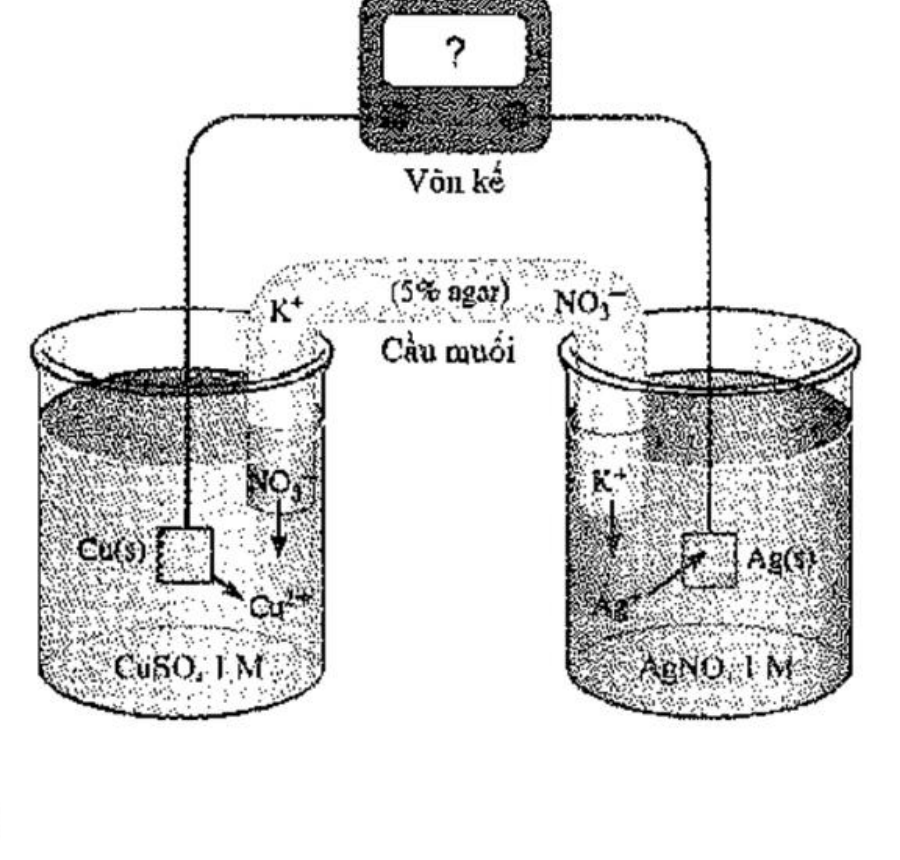
\includegraphics[height=2.3cm]{images_crop_de13/p2_cau2_pin_cu_ag.png}\par}\vspace{2pt}
\choiceTF
{\True Giá trị sức điện động chuẩn của pin điện hoá trên là 0,459 V}
{\True Ở anode xảy ra quá trình oxi hoá Cu, ở cathode xảy ra quá trình khử \ce{Ag+}}
{Điện cực Cu tăng khối lượng, điện cực Ag giảm khối lượng}
{\True Phản ứng hoá học xảy ra trong pin: \ce{Cu + 2Ag+ -> Cu^2+ + 2Ag}}
\loigiai{
a) \textbf{Đúng}. $E^\circ_{\text{pin}} = E^\circ_{\ce{Ag+/Ag}} - E^\circ_{\ce{Cu^2+/Cu}} = 0{,}799 - 0{,}340 = 0{,}459\text{ V}$.\\
b) \textbf{Đúng}. Cực Cu có thế điện cực nhỏ hơn nên là anode (xảy ra oxi hóa Cu: \ce{Cu -> Cu^2+ + 2e}), cực Ag là cathode (xảy ra khử \ce{Ag+}: \ce{Ag+ + 1e -> Ag}).\\
c) \textbf{Sai}. Ở anode Cu bị tan ra nên khối lượng cực Cu giảm; ở cathode Ag bám vào nên khối lượng cực Ag tăng.\\
d) \textbf{Đúng}. Phản ứng tổng quát chuẩn xảy ra trong pin: \ce{Cu + 2Ag+ -> Cu^2+ + 2Ag}.}
\end{ex}

\begin{ex}
Thí nghiệm điện phân được thực hiện như hình vẽ sau:
\par\vspace{2pt}{\centering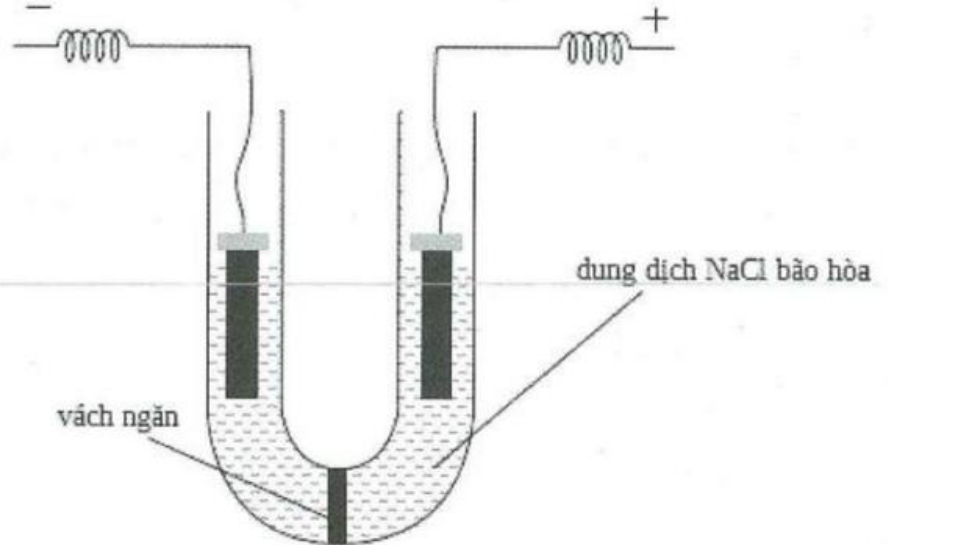
\includegraphics[height=2.1cm]{images_crop_de13/p2_cau3_dien_phan_nacl.png}\par}\vspace{2pt}
\choiceTF
{Có khí \ce{H2} thoát ra ở điện cực dương, khí \ce{O2} thoát ra ở cực âm}
{\True Thí nghiệm này ứng dụng để điều chế \ce{NaOH} trong công nghiệp}
{\True Nếu không có vách ngăn điện cực, dung dịch thu được có tính tẩy màu}
{\True Dung dịch sau điện phân làm quỳ tím chuyển sang màu xanh}
\loigiai{
a) \textbf{Sai}. Ở cực âm (cathode) thoát khí \ce{H2}; ở cực dương (anode) thoát khí \ce{Cl2}.\\
b) \textbf{Đúng}. Đây là mô hình điện phân dung dịch \ce{NaCl} bão hòa có màng ngăn điều chế \ce{NaOH}, \ce{Cl2}, \ce{H2} công nghiệp.\\
c) \textbf{Đúng}. Không có màng ngăn, \ce{Cl2} tác dụng với \ce{NaOH} tạo nước Javel (\ce{NaClO}) có tính tẩy màu.\\
d) \textbf{Đúng}. Dung dịch chứa \ce{NaOH} là base mạnh làm quỳ tím hóa xanh.}
\end{ex}

\begin{ex}
Điện phân dung dịch \ce{MSO4} (M là kim loại) với điện cực trơ, cường độ dòng điện không đổi. Sau thời gian $t$ giây, thu được $a\text{ mol}$ khí ở anode. Nếu thời gian điện phân là $2t$ giây thì tổng số mol khí thu được ở cả hai điện cực là $2{,}5a\text{ mol}$. Giả sử hiệu suất điện phân là 100\%, khí sinh ra không tan trong nước.
\choiceTF
{\True Tại thời điểm $2t$ giây, có bọt khí ở cathode}
{\True Tại thời điểm $t$ giây, ion \ce{M^2+} chưa bị điện phân hết}
{\True Dung dịch sau điện phân có pH $< 7$}
{Khi thu được $1{,}8a\text{ mol}$ khí ở anode thì vẫn chưa xuất hiện bọt khí ở cathode}
\loigiai{
- Tại $t$ giây: Ở anode thoát $a\text{ mol } \ce{O2} \Rightarrow n_e = 4a\text{ mol}$.\\
- Tại $2t$ giây: $n_e = 8a\text{ mol} \Rightarrow n_{\ce{O2}} = 2a\text{ mol}$. Tổng mol khí ở cả hai cực là $2{,}5a \Rightarrow n_{\ce{H2}\text{ (cathode)}} = 0{,}5a\text{ mol}$.\\
$\Rightarrow$ Ý a \textbf{Đúng}.\\
- Bảo toàn electron tại $2t$ giây: $2n_{\ce{M^2+}} + 2n_{\ce{H2}} = 8a \Rightarrow 2n_{\ce{M^2+}} = 7a \Rightarrow n_{\ce{M^2+}} = 3{,}5a\text{ mol}$.\\
Tại $t$ giây lượng \ce{M^2+} tham gia khử là $2a < 3{,}5a\text{ mol}$, nên ion \ce{M^2+} chưa điện phân hết $\Rightarrow$ Ý b \textbf{Đúng}.\\
- Lượng \ce{H+} sinh ra ở anode ($4 \times 2a = 8a\text{ mol}$) nhiều hơn lượng \ce{OH-} sinh ra ở cathode ($2 \times 0{,}5a = 1a\text{ mol}$) $\Rightarrow$ dung dịch có tính acid ($\text{pH} < 7$) $\Rightarrow$ Ý c \textbf{Đúng}.\\
- Khi anode thoát $1{,}8a\text{ mol } \ce{O2} \Rightarrow n_e = 7{,}2a\text{ mol}$. Lượng $n_e$ để khử hết \ce{M^2+} là $2 \times 3{,}5a = 7{,}0a < 7{,}2a \Rightarrow$ Đã có bọt khí \ce{H2} thoát ra ở cathode $\Rightarrow$ Ý d \textbf{Sai}.}
\end{ex}



\noindent
\textbf{PHẦN III (1,5 điểm -- 6 câu): Câu trắc nghiệm yêu cầu trả lời ngắn.}\\
\textit{Thí sinh trả lời từ câu 1 đến câu 6.}

\setcounter{ex}{0}

\begin{ex}
Có 3 cốc đựng các dung dịch muối có nồng độ 1 M, cho vào mỗi cốc 1 thanh Al:\\
(a) Cốc I: \ce{Pb(NO3)2} (aq)\quad (b) Cốc II: \ce{Ni(NO3)2} (aq)\quad (c) Cốc III: \ce{Cu(NO3)2} (aq)\\
Có bao nhiêu cốc có phản ứng xảy ra?
\par\noindent\textbf{Đáp số:} \textbf{\color{red}3}
\loigiai{
Thế điện cực chuẩn của Al: $E^\circ_{\ce{Al^3+/Al}} = -1{,}66\text{ V}$ nhỏ hơn cả ba cặp \ce{Pb^2+/Pb} ($-0{,}13\text{ V}$), \ce{Ni^2+/Ni} ($-0{,}26\text{ V}$) và \ce{Cu^2+/Cu} ($+0{,}34\text{ V}$).\\
Do đó kim loại Al có tính khử mạnh hơn và đẩy được cả 3 kim loại Pb, Ni, Cu ra khỏi dung dịch muối của chúng. Cả 3 cốc đều xảy ra phản ứng.\\
\textbf{Đáp số: 3.}}
\end{ex}

\begin{ex}
Cho pin điện hóa Zn -- Cu gồm hai cặp oxi hóa -- khử \ce{Zn^2+/Zn} và \ce{Cu^2+/Cu}. Cho thế điện cực chuẩn $E^\circ_{\ce{Cu^2+/Cu}} = 0{,}34\text{ V}$ và $E^\circ_{\ce{Zn^2+/Zn}} = -0{,}76\text{ V}$. Tính sức điện động chuẩn của pin (theo đơn vị V).
\par\noindent\textbf{Đáp số:} \textbf{\color{red}1,1}
\loigiai{
Sức điện động chuẩn của pin điện hoá Zn -- Cu là:
$$E^\circ_{\text{pin}} = E^\circ_{\ce{Cu^2+/Cu}} - E^\circ_{\ce{Zn^2+/Zn}} = 0{,}34 - (-0{,}76) = 1{,}10\text{ V.}$$
\textbf{Đáp số: 1,1.}}
\end{ex}

\begin{ex}
Điện phân dung dịch hỗn hợp gồm: \ce{NaCl}, \ce{Mg(NO3)2}, \ce{ZnCl2}, \ce{CuSO4} và \ce{Fe2(SO4)3} với điện cực trơ cho đến khi nước bắt đầu điện phân ở cả hai điện cực thì dừng lại. Thu được bao nhiêu chất rắn (kim loại) ở cathode?
\par\noindent\textbf{Đáp số:} \textbf{\color{red}3}
\loigiai{
Tại cathode (cực âm), thứ tự nhận electron theo chiều giảm dần tính oxi hoá của các cation:\\
1. \ce{Fe^3+ + 1e -> Fe^2+}.\\
2. \ce{Cu^2+ + 2e -> Cu}$\downarrow$ (chất rắn 1).\\
3. \ce{Fe^2+ + 2e -> Fe}$\downarrow$ (chất rắn 2).\\
4. \ce{Zn^2+ + 2e -> Zn}$\downarrow$ (chất rắn 3).\\
Các cation \ce{Mg^2+}, \ce{Na+} không bị khử trong dung dịch nước. Sau khi \ce{Zn^2+} khử hết thì nước bị điện phân thoát khí \ce{H2}.\\
Vậy thu được 3 kim loại bám ở cathode là Cu, Fe và Zn.\\
\textbf{Đáp số: 3.}}
\end{ex}

\begin{ex}
Cho các phản ứng sau:\\
(1) Cho Cu vào dung dịch \ce{FeSO4}.\\
(2) Cho Cu vào dung dịch \ce{Fe2(SO4)3}.\\
(3) Cho K vào dung dịch \ce{CuSO4}.\\
(4) Cho dung dịch \ce{AgNO3} vào dung dịch \ce{Fe(NO3)2}.\\
Số lượng phản ứng có thể thu được đơn chất kim loại là
\par\noindent\textbf{Đáp số:} \textbf{\color{red}1}
\loigiai{
- (1) Cu không phản ứng với \ce{FeSO4} vì tính khử $\text{Cu} < \text{Fe}$.\\
- (2) \ce{Cu + Fe2(SO4)3 -> CuSO4 + 2FeSO4} (không sinh ra kim loại).\\
- (3) Kim loại kiềm K phản ứng với nước trước tạo KOH, sau đó tạo kết tủa \ce{Cu(OH)2} (không thu được kim loại Cu).\\
- (4) \ce{AgNO3 + Fe(NO3)2 -> Fe(NO3)3 + Ag}$\downarrow$ (thu được kim loại Ag).\\
Vậy chỉ có 1 phản ứng thu được đơn chất kim loại.\\
\textbf{Đáp số: 1.}}
\end{ex}

\begin{ex}
Cho một pin Galvani với điện cực Zn và Cu có sức điện động chuẩn là 1,10 V. Sử dụng pin này để thắp sáng một bóng đèn nhỏ với cường độ dòng điện chạy qua là $I = 0{,}02\text{ A}$. Nếu điện cực kẽm hao mòn 0,1 mol do pin phóng điện thì thời gian tối đa mà pin thắp sáng được bóng đèn là bao nhiêu giờ?\\
Cho biết công thức: $Q = n \cdot F = I \cdot t$, trong đó $Q$ là điện lượng (C), $n$ là số mol electron đi qua dây dẫn, $I$ là cường độ dòng điện (A), $t$ là thời gian (giây), $F$ là hằng số Faraday ($F = 96500\text{ C/mol}$). (Làm tròn kết quả đến hàng đơn vị).
\par\noindent\textbf{Đáp số:} \textbf{\color{red}268}
\loigiai{
Quá trình xảy ra ở anode: \ce{Zn -> Zn^2+ + 2e}.\\
Số mol electron giải phóng khi tiêu hao $0{,}1\text{ mol}$ Zn là:
$$n_e = 2 \times n_{\ce{Zn}} = 2 \times 0{,}1 = 0{,}2\text{ mol.}$$
Điện lượng sinh ra:
$$Q = n_e \times F = 0{,}2 \times 96500 = 19300\text{ C.}$$
Thời gian thắp sáng bóng đèn:
$$t = \frac{Q}{I} = \frac{19300}{0{,}02} = 965000\text{ giây.}$$
Đổi ra giờ:
$$t = \frac{965000}{3600} \approx 268{,}06 \approx 268\text{ giờ.}$$
\textbf{Đáp số: 268.}}
\end{ex}

\begin{ex}
Tiến hành điện phân dung dịch \ce{CuSO4} với anode bằng đồng (hiện tượng dương cực tan). Để hoà tan $100\text{ g}$ đồng ở anode trong 8 giờ thì cần cường độ dòng điện bằng bao nhiêu ampe? (Làm tròn kết quả đến chữ số hàng phần mười).
\par\noindent\textbf{Đáp số:} \textbf{\color{red}10,5}
\loigiai{
Số mol đồng bị hòa tan ở anode:
$$n_{\ce{Cu}} = \frac{100}{64} = 1{,}5625\text{ mol.}$$
Quá trình tại anode: \ce{Cu -> Cu^2+ + 2e} $\Rightarrow n_e = 2 \times n_{\ce{Cu}} = 3{,}125\text{ mol}$.\\
Điện lượng cần cung cấp:
$$Q = n_e \times F = 3{,}125 \times 96500 = 301562{,}5\text{ C.}$$
Thời gian điện phân đổi sang giây:
$$t = 8 \times 3600 = 28800\text{ giây.}$$
Cường độ dòng điện cần dùng:
$$I = \frac{Q}{t} = \frac{301562{,}5}{28800} \approx 10{,}47 \approx 10{,}5\text{ A.}$$
\textbf{Đáp số: 10,5.}}
\end{ex}


\Closesolutionfile{ans}

\vspace{0.5cm}
\begin{center}
	\textbf{\Large\color{mainGreen}BẢNG TỔNG HỢP ĐÁP ÁN ĐỀ SỐ 13}
\end{center}

\vspace{0.2cm}
\noindent\textbf{\color{mainGreen}PHẦN I: TRẮC NGHIỆM NHIỀU PHƯƠNG ÁN LỰA CHỌN}
\begin{center}
\renewcommand{\arraystretch}{1.2}
\begin{tabular}{|c|c|c|c|c|c|c|c|c|c|c|c|c|c|c|c|c|c|}
\hline
\textbf{1} & \textbf{2} & \textbf{3} & \textbf{4} & \textbf{5} & \textbf{6} & \textbf{7} & \textbf{8} & \textbf{9} & \textbf{10} & \textbf{11} & \textbf{12} & \textbf{13} & \textbf{14} & \textbf{15} & \textbf{16} & \textbf{17} & \textbf{18} \\ \hline
\textbf{\color{red}A} & \textbf{\color{red}A} & \textbf{\color{red}A} & \textbf{\color{red}D} & \textbf{\color{red}B} & \textbf{\color{red}A} & \textbf{\color{red}B} & \textbf{\color{red}B} & \textbf{\color{red}B} & \textbf{\color{red}A} & \textbf{\color{red}B} & \textbf{\color{red}D} & \textbf{\color{red}D} & \textbf{\color{red}D} & \textbf{\color{red}B} & \textbf{\color{red}D} & \textbf{\color{red}D} & \textbf{\color{red}D} \\ \hline
\end{tabular}
\end{center}

\vspace{0.3cm}
\noindent\textbf{\color{mainGreen}PHẦN II: TRẮC NGHIỆM ĐÚNG SAI}
\begin{center}
\renewcommand{\arraystretch}{1.2}
\begin{tabular}{|c|c|c|c|c|}
\hline
\textbf{Câu} & \textbf{Lệnh hỏi a} & \textbf{Lệnh hỏi b} & \textbf{Lệnh hỏi c} & \textbf{Lệnh hỏi d} \\ \hline
\textbf{1} & \textbf{\color{red}Đ} & \textbf{\color{red}Đ} & \textbf{\color{red}Đ} & \textbf{\color{red}Đ} \\ \hline
\textbf{2} & \textbf{\color{red}Đ} & \textbf{\color{red}Đ} & \textbf{S} & \textbf{\color{red}Đ} \\ \hline
\textbf{3} & \textbf{S} & \textbf{\color{red}Đ} & \textbf{\color{red}Đ} & \textbf{\color{red}Đ} \\ \hline
\textbf{4} & \textbf{\color{red}Đ} & \textbf{\color{red}Đ} & \textbf{\color{red}Đ} & \textbf{S} \\ \hline
\end{tabular}
\end{center}

\vspace{0.3cm}
\noindent\textbf{\color{mainGreen}PHẦN III: TRẢ LỜI NGẮN}
\begin{center}
\renewcommand{\arraystretch}{1.2}
\begin{tabular}{|c|c|c|c|c|c|}
\hline
\textbf{Câu 1} & \textbf{Câu 2} & \textbf{Câu 3} & \textbf{Câu 4} & \textbf{Câu 5} & \textbf{Câu 6} \\ \hline
\textbf{\color{red}3} & \textbf{\color{red}1,1} & \textbf{\color{red}3} & \textbf{\color{red}1} & \textbf{\color{red}268} & \textbf{\color{red}10,5} \\ \hline
\end{tabular}
\end{center}

\end{document}
